\documentclass{beamer}
\mode<presentation>
\usetheme{Madrid}
\usecolortheme{crane}

\usepackage{tikz}
\usepackage{epic}
\usepackage{qtree}
\usepackage[normalem]{ulem}
\usepackage{tikz-dependency}

\title{N-grams and smoothing; or, how language is (a bit) like the weather}
\subtitle{Language Technology I}
\author{Asad Sayeed}
\institute{Saarland University}
\date{}

\setbeamertemplate{navigation symbols}{}

\newcommand{\placard}[1]{
  \begin{frame}
    \begin{center}
      \huge
      \textbf{#1}
    \end{center}
  \end{frame}
}

\newcommand{\pagestep}[2]{
  \begin{frame}[t]
    \begin{minipage}[t][0.26\textheight][t]{\textwidth}
      \begin{center}
        \huge
        \textbf{#1}
      \end{center}
    \end{minipage}
    
    \begin{minipage}[t][0.7\textheight][c]{\textwidth}
      \begin{center}
        \includegraphics[height=0.83\textheight]{#2}
      \end{center}
    \end{minipage}
  \end{frame}
}

\newcommand{\pagestepalt}[2]{
  \begin{frame}[t]
    \begin{minipage}[t][0.26\textheight][t]{\textwidth}
      \begin{center}
        \huge
        \textbf{#1}
      \end{center}
    \end{minipage}
    
    \begin{minipage}[t][0.7\textheight][t]{\textwidth}
      #2
    \end{minipage}
  \end{frame}
}


\begin{document}
\makeatletter
\setbeamertemplate{footline}
{
  \leavevmode%
  \hbox{%
  \begin{beamercolorbox}[wd=.333333\paperwidth,ht=2.25ex,dp=1ex,center]{author in head/foot}%
    \usebeamerfont{author in head/foot}\insertshortauthor\expandafter\beamer@ifempty\expandafter{\beamer@shortinstitute}{}{~~(\insertshortinstitute)}
  \end{beamercolorbox}%
  \begin{beamercolorbox}[wd=.333333\paperwidth,ht=2.25ex,dp=1ex,center]{title in head/foot}%
    \usebeamerfont{title in head/foot}\insertshorttitle
  \end{beamercolorbox}%
  \begin{beamercolorbox}[wd=.333333\paperwidth,ht=2.25ex,dp=1ex,right]{date in head/foot}%
    \usebeamerfont{date in head/foot}\insertshortdate{}\hspace*{2em}
%    \insertframenumber{} / \inserttotalframenumber\hspace*{2ex} 
    \insertframenumber{}\hspace*{2ex}
    \hspace*{6ex}
  \end{beamercolorbox}}%
  \vskip0pt%
}
\makeatother


\begin{frame}
  \titlepage
\end{frame}

% \pagestepalt{\textcolor{blue}{Meta-comments.}}{
%   {\color{blue}
%     As this is a simulation/isn't a full-length class, I will
%       mention class activities in blue but not run through them.  
%   }
% }

\pagestepalt{Objectives for today}{
  \begin{enumerate}
  \item Explore the idea of sequences in language (n-grams). 
  \item Consider sequences as models of probability.
  \item Handle the prediction of unseen items (smoothing).
  \end{enumerate}
}

\placard{Q: Does language have anything to do with the weather?}

\placard{A: Yes. But first\ldots}

\pagestepalt{\ldots a tongue-twister in English.}{
  \begin{center}
    \Large How much wood could a woodchuck chuck if a woodchuck could
    chuck wood?
  \end{center}\pause
  One possible answer:
  \begin{center}
    \Large As much wood as a woodchuck could chuck. 
  \end{center}
}

\pagestepalt{Can we calculate how \alert{likely} that answer is?}{
  \pause That depends \ldots on what you mean by ``likely''.\pause\\ To
  estimate the likelihood of an answer (in the form of a sentence),
  you need:
  \begin{itemize}
  \item An evidentiary basis.
    \\$\Rightarrow$ in modern \alert{statistical} natural language processing,
    we use large \alert{corpora}. \pause 
  \item A theory that connects the evidence to the likelihood you're
    trying to estimate.  \pause
    \begin{itemize}
    \item Assume sentences are made of words.  
    \item So the probability of a sentence might have something 
      to do with the probability of the words in the sentence.
    \end{itemize}\pause
  \item A means to combine the pieces of evidence.\\
    $\Rightarrow$ if words matter, then we need a \alert{theory} of sentence
    structure from words.
  \end{itemize}
}

\pagestepalt{Why do we want a likelihood?}{
%  \textcolor{blue}{[Solicit answers from students.]}\\ \pause
  Consider natural language processing systems in real life. E.g., machine 
  translation:
  \begin{itemize}
  \item Translate ``How much wood \alert{could} a woodchuck chuck?'' to French.
    \begin{itemize}
    \item The word ``could'': possibility in French expressible with 
      two different grammatical forms ({\it ``peut''/``pourrait''}).
    \item Choose better one {\it in context}.
    \item Hard to do over all words deterministically $\leftarrow$
      years of effort to create the ``rules'', but never succeed.
    \end{itemize}
  \item Countless other applications: such as answering a question\ldots.
  \end{itemize}
}

\pagestepalt{So how do we get the evidence?}{
  Count words.
  \begin{center}
    \Large how much wood could a woodchuck chuck if a woodchuck could
    chuck wood ?
  \end{center}
  Assume that this is our corpus. Total number of words: 14 (incl. the ``?'').
%  \\ \textcolor{blue}{[Get students to follow along.]}\pause
  \only<2>{\vspace{-0.75cm}\begin{columns}[T]
      \begin{column}{0.5\textwidth}
        \begin{center}
          \small
          \begin{tabular}{c|c}
            word type & token count \\
            \hline
            a & 2 \\
            chuck & 2 \\
            could & 2 \\
            how & 1 \\
            if & 1 \\
          \end{tabular}
        \end{center}
      \end{column}
      \begin{column}{0.5\textwidth}
        \begin{center}
          \small
          \begin{tabular}{c|c}
            word type & token count \\
            \hline
            much & 1 \\
            wood & 2 \\
            woodchuck & 2 \\
            ? & 1 \\
          \end{tabular}
        \end{center}
      \end{column}
  \end{columns}}
  \only<3>{\vspace{-0.75cm}\begin{columns}[T]
      \begin{column}{0.5\textwidth}
        \begin{center}
          \small
          \begin{tabular}{c|c|c}
            word type & token count & \alert{p(word)}\\
            \hline
            a & 2 & 0.14\\
            chuck & 2 & 0.14 \\
            could & 2 & 0.14 \\
            how & 1 & 0.07\\
            if & 1 & 0.07 \\
          \end{tabular}
        \end{center}
      \end{column}
      \begin{column}{0.5\textwidth}
        \begin{center}
          \small
          \begin{tabular}{c|c|c}
            word type & token count & \alert{p(word)} \\
            \hline
            much & 1 & 0.07\\
            wood & 2 & 0.14 \\
            woodchuck  &2 & 0.14 \\
            ? & 1 & 0.07 \\
          \end{tabular}
        \end{center}
      \end{column}
  \end{columns}
  Then calculate probability per \alert{type} of word as count/14.
  }


  %% \only<2>{\begin{center}
  %%   \begin{tabular}{c|c|c}
  %%     word & count & \alert{p(word)}\\
  %%     \hline
  %%     a & 2 & 0.14\\
  %%     chuck & 2 & 0.14 \\
  %%     could & 2 & 0.14 \\
  %%     how & 1 & 0.07\\
  %%     if & 1 & 0.07 \\
  %%   \end{tabular}
  %%   \begin{tabular}{c|c|c}
  %%     word & count & \alert{p(word)} \\
  %%     \hline
  %%     much & 1 & 0.07\\
  %%     wood & 2 & 0.14 \\
  %%     woodchuck 2 & & 0.14 \\
  %%     ? & 1 & 0.07 \\
  %%   \end{tabular}
  %% \end{center}
  %% Then calculate probability per \alert{type} of word as count/14.
  %% }
}

\pagestepalt{Calculate the probability of expressions.}{
  \vspace{-1cm}
  \begin{columns}[T]
    \begin{column}{0.5\textwidth}
      \begin{center}
        \small
        \begin{tabular}{c|c|c}
          word type & token count & \alert{p(word)}\\
          \hline
          a & 2 & 0.14\\
          chuck & 2 & 0.14 \\
          could & 2 & 0.14 \\
          how & 1 & 0.07\\
          if & 1 & 0.07 \\
        \end{tabular}
      \end{center}
    \end{column}
    \begin{column}{0.5\textwidth}
      \begin{center}
        \small
        \begin{tabular}{c|c|c}
          word type & token count & \alert{p(word)} \\
          \hline
          much & 1 & 0.07\\
          wood & 2 & 0.14 \\
          woodchuck  &2 & 0.14 \\
          ? & 1 & 0.07 \\
        \end{tabular}
      \end{center}
    \end{column}
  \end{columns}
  The \alert{joint probability} of multiple words: how likely they are to occur
  in the same text.
  \begin{block}{}
    $p(w_1,w_2,\ldots) = p(w_1)p(w_2)\ldots$
  \end{block}
  Calculate some conditional probabilities:
% \textcolor{blue}{[student activity]}:
  \begin{itemize}
    \item $p($if,woodchuck$)=$ \only<2>{\alert{0.07 x 0.14 = 0.01} }
    \item $p($wood,woodchuck$)=$ \only<2>{\alert{0.14 x 0.14 = 0.02}}
    \item $p($how,could,a$)=$ \only<2>{\alert{0.07 x 0.14 x 0.14 = 0.001}}
  \end{itemize}
}

\pagestepalt{Calculating the probability of expressions.}{
  \vspace{-1cm}
  \begin{columns}[T]
    \begin{column}{0.5\textwidth}
      \begin{center}
        \small
        \begin{tabular}{c|c|c}
          word type & token count & \alert{p(word)}\\
          \hline
          a & 2 & 0.14\\
          chuck & 2 & 0.14 \\
          could & 2 & 0.14 \\
          how & 1 & 0.07\\
          if & 1 & 0.07 \\
        \end{tabular}
      \end{center}
    \end{column}
    \begin{column}{0.5\textwidth}
      \begin{center}
        \small
        \begin{tabular}{c|c|c}
          word type & token count & \alert{p(word)} \\
          \hline
          much & 1 & 0.07\\
          wood & 2 & 0.14 \\
          woodchuck  &2 & 0.14 \\
          ? & 1 & 0.07 \\
        \end{tabular}
      \end{center}
    \end{column}
  \end{columns}
  Now we can calculate the joint probability of our answer.
  \begin{center}
    \Large As much wood as a woodchuck could chuck. 
  \end{center}
  \begin{itemize}
  \item $p($as,much,wood,as,a,woodchuck,could,chuck$)$ = \pause \alert{0 x \ldots}\pause
  \item Uh oh: there's no ``as'' in our probability table. \\
    $\Rightarrow$ we will get to missing items soon.\pause
  \item So, try $p($much,wood,a,woodchuck,could,chuck$)$ = \\ \pause \alert{0.07 x 0.14 x 0.14 x 0.14 x 0.14 x 0.14  = 3.76e-05}
  \end{itemize}
}

\pagestepalt{Words come in an order.}{
  Calculating the joint probability of \alert{unigrams} (single words):
  is it a good \alert{model}?\pause \\
  Backwards\ldots
  \begin{center}
    \Large chuck could woodchuck a as wood much as
  \end{center}
  \ldots is not an English sentence. \pause
  \begin{itemize}
  \item Joint unigram probability: the same, no matter what, as ``as much wood as a woodchuck could chuck''.\pause
  \item We definitely don't want that to be true.  So our theory must include
    sequences.
  \end{itemize}
}

\placard{And this is what language has to do with the weather.}

\pagestepalt{What was the weather like two years ago in Holland?}{
  Average temperature at Amsterdam Schiphol:\\
  \begin{flushright}
    \begin{tabular}{|c|}
      \hline
      18.11.2014 \\
      {\Huge 8 C} \\
      \hline
   \end{tabular}
  \end{flushright}
}

\pagestepalt{And what was it the day before that?}{
  Average temperature at Amsterdam Schiphol:\\
  \begin{flushright}
    \begin{tabular}{|c|}
      \hline
      17.11.2014 \\
      {\Huge 10 C} \\
      \hline
    \end{tabular}
    \begin{tabular}{|c|}
      \hline
      18.11.2014 \\
      {\Huge 8 C} \\
      \hline
    \end{tabular}
  \end{flushright}
}

\pagestepalt{And before that?}{
  Average temperature at Amsterdam Schiphol:\\
  \begin{flushright}
    \begin{tabular}{|c|}
      \hline
      16.11.2014 \\
      {\Huge 9 C} \\
      \hline
    \end{tabular}
    \begin{tabular}{|c|}
      \hline
      17.11.2014 \\
      {\Huge 10 C} \\
      \hline
    \end{tabular}
    \begin{tabular}{|c|}
      \hline
      18.11.2014 \\
      {\Huge 8 C} \\
      \hline
    \end{tabular}
  \end{flushright}
}


\placard{It's as though we know something about the next day from the
  previous days!}

\placard{But how many days do we need?}

\pagestepalt{Surely not to the beginning of the Earth!}{
  Average temperature at Amsterdam Schiphol:\\
  \begin{flushright}
    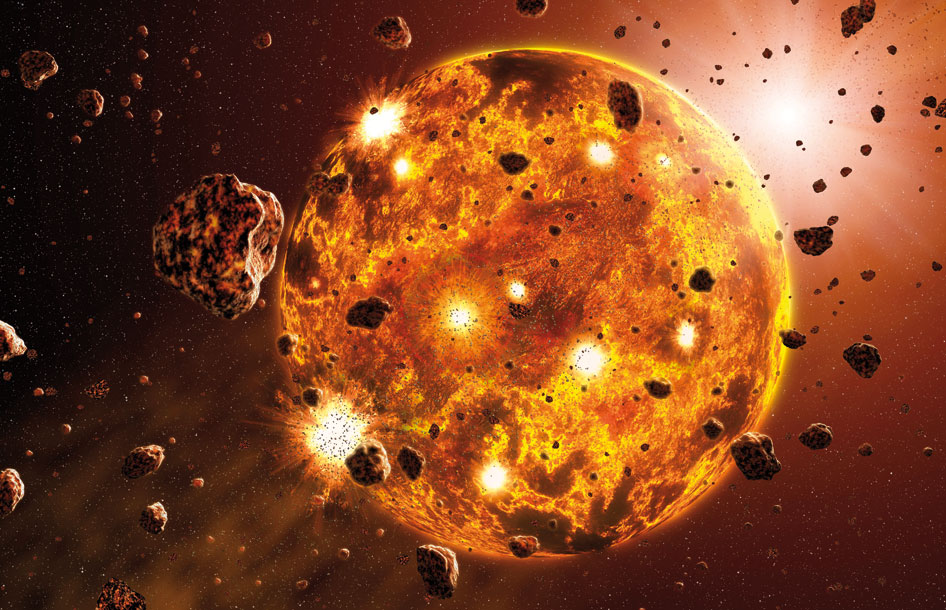
\includegraphics[width=0.3\textwidth]{images/formation.jpg}
    {\Huge\ldots}
    \begin{tabular}{|c|}
      \hline
      16.11.2014 \\
      {\Huge 9 C} \\
      \hline
    \end{tabular}
    \begin{tabular}{|c|}
      \hline
      17.11.2014 \\
      {\Huge 10 C} \\
      \hline
    \end{tabular}
    \begin{tabular}{|c|}
      \hline
      18.11.2014 \\
      {\Huge 8 C} \\
      \hline
    \end{tabular}
  \end{flushright}
}
\pagestepalt{We have expectations about changes.}{
  We know that yesterday is a good clue about today. \\
  Temperatures in Amsterdam in 2014:
  \begin{center}
    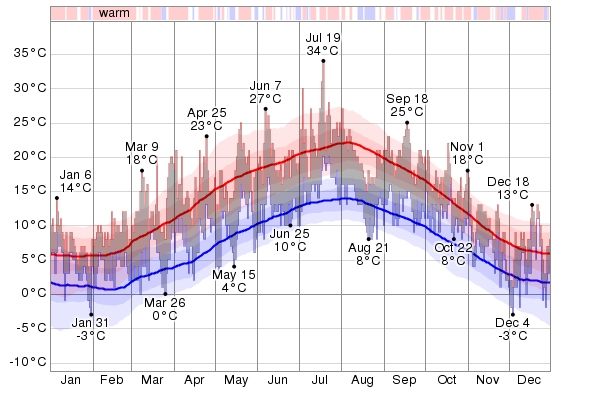
\includegraphics[width=0.70\textwidth]{images/amstemp.png}
  \end{center}
}

\pagestepalt{The daily temperature is a \alert{Markov process}.}{
  Let $T_d=$ temperature $T$ on day $d$.\\
  We can represent the probability conditionally.
  \begin{block}{Probability of today's temperature \only<1>{given universe}\only<2->{\alert{given 2 previous days}}}
    $p(T_d|T_{d-1},T_{d-2},\ldots,T_{d-\infty})$ \only<2->{\alert{$\approx p(T_d|T_{d-1},T_{d-2})$}}
  \end{block}\pause
  But we only need a few days to give us a trend. So we make a 
  \alert{Markov assumption}.\\ \pause
  Then we can calculate the joint probability of a sequence of days:
  \begin{block}{\alert{Markov chain}}
    $p(T_d,T_{d-1},T_{d-2}) = p(T_d|T_{d-1},T_{d-2})p(T_{d-1}|T_{d-2},T_{d-3})p(T_{d-2}|T_{d-3},T_{d-4})$
  \end{block}
}


 
%% \pagestepalt{But that's the same with language.}{
%%   When we see the word\ldots
%%   \begin{block}{}
%%     \begin{center}
%%       \Huge
%%       the \only<2-3>{the} 
%%     \end{center}
%%   \end{block}\pause
%%   we don't expect it (in text) to be followed by a second
%%   one.\\ \pause But that's an extreme case (where it's ungrammatical).
%% }

%% \pagestepalt{But more commonly\ldots}{
%%   \ldots even grammatical pairs of words are differently likely.
%%   \begin{block}{}
%%     \begin{center}
%%       {\Huge      $p$(``the fish'') $> p$(``the fowl'')}
%%     \end{center}
%%   \end{block}
%%   Trust me, I checked.
%% }

\pagestepalt{Getting Markovian with language.}{
  Let's make a Markov assumption over sentences. So how many words previous
  to ``chuck'' do we need?
  \begin{center}
    \Large As \alert<4>{much} wood as a \alert<3->{woodchuck} \alert<2->{could} \textbf{chuck}. 
  \end{center}
%  \textcolor{blue}{[student discussion]}
  \pause
  \begin{itemize}
  \item ``could'' is an auxiliary that selects for a verb.\pause
  \item ``woodchuck'' -- maybe. We're asking if woodchucks can chuck, it's in the corpus.\pause
  \item ``much''? No, probably not.
  \end{itemize}\pause
  Two words back seems to be a common choice.
}

\pagestepalt{We can check a bigger corpus.}{
  Leave aside the woodchucks for a moment. Let's try a couple of 2-word
  expressions. ``The fish'' vs ``the fowl.''.\\
  The Google Books Ngram viewer:
  \begin{center}
    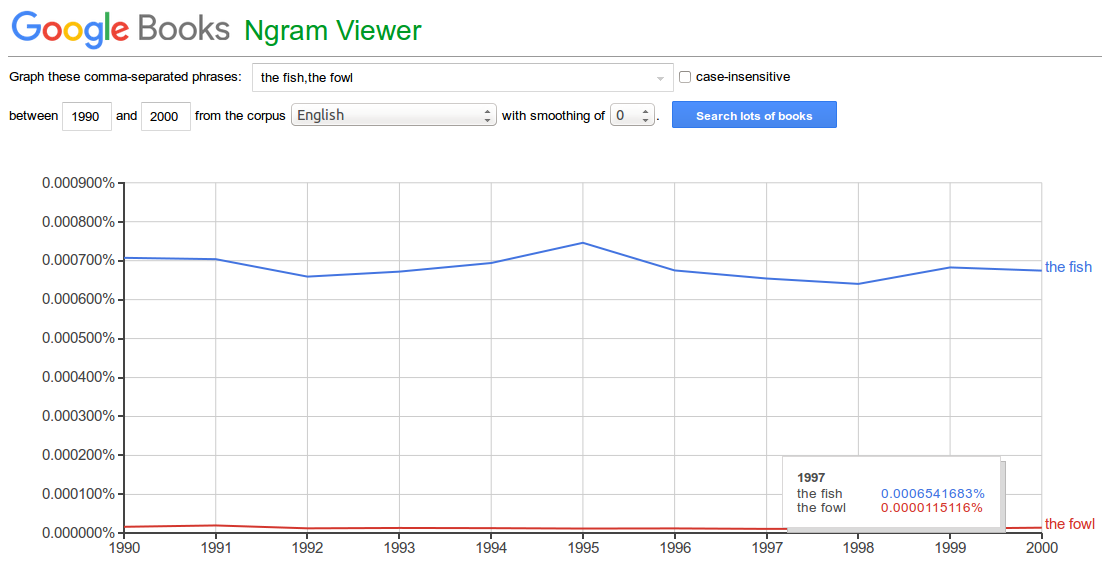
\includegraphics[width=0.75\textwidth]{images/fishvfowl.png}
  \end{center}
}

\pagestepalt{But lots of things follow ``the''.}{
  \begin{center}
    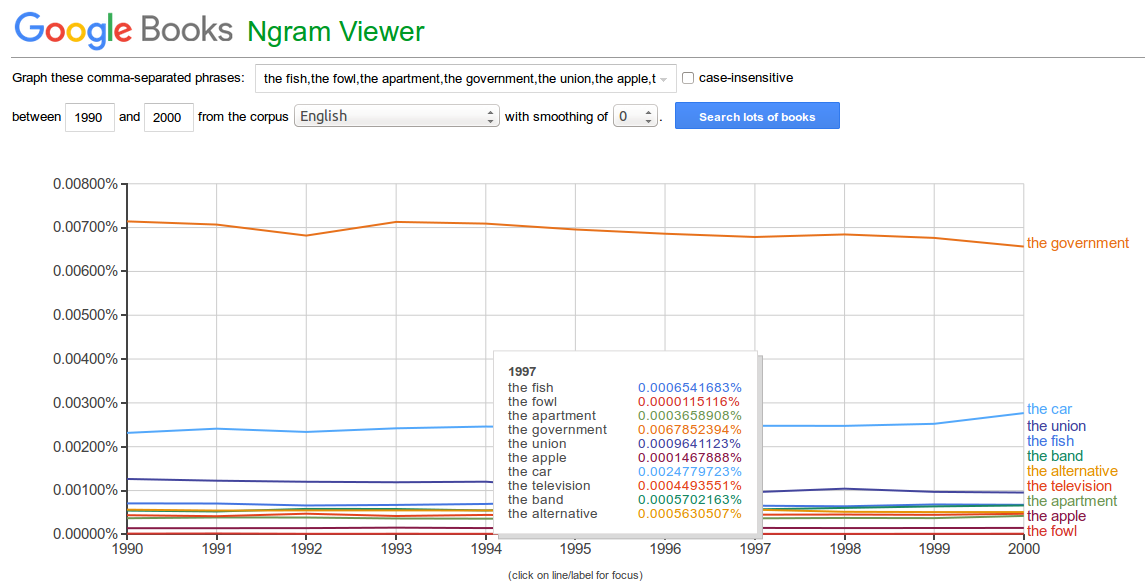
\includegraphics[width=0.8\textwidth]{images/fishvlots.png}
  \end{center}
}

\pagestepalt{It's not hugely informative\ldots}{
  \ldots because the whole category of nouns can follow ``the''.\\ \pause
  So what if we add another word, ``eat'':
  \begin{center}
    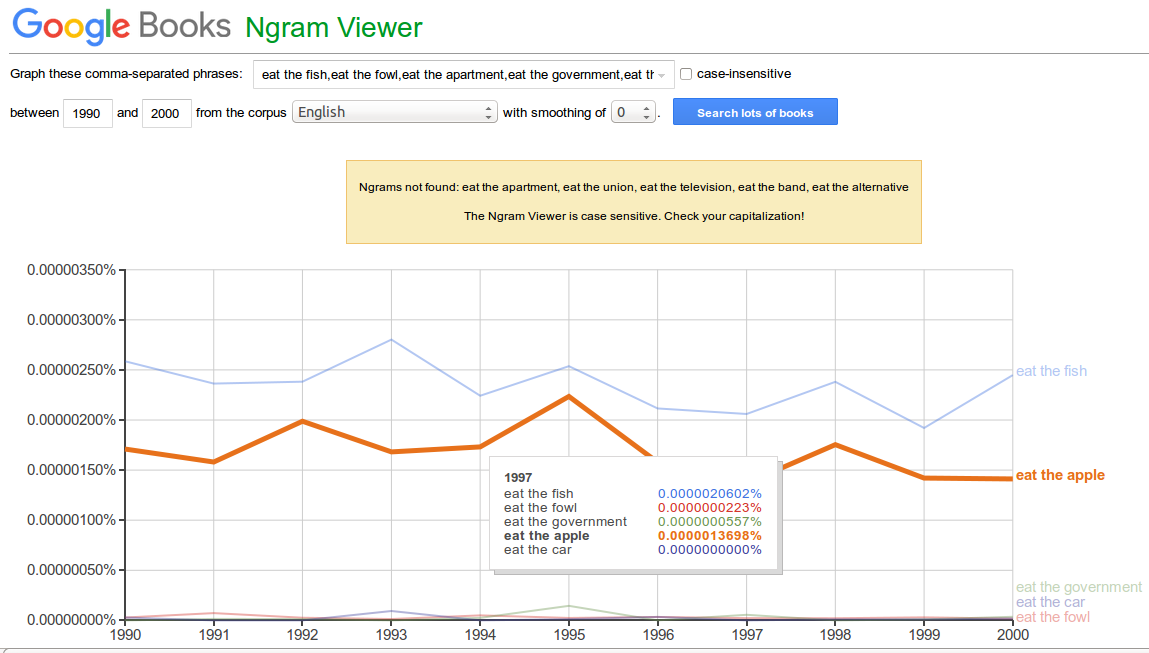
\includegraphics[width=0.75\textwidth]{images/eat.png}
  \end{center}
}

\pagestepalt{The additional word is hugely informative!}{
  So this is a way language is \textbf{not} like the weather.\pause
  \begin{itemize}
  \item Sure, tomorrow will resemble today, in terms of temperature.
    \begin{itemize}
    \item But knowing what happened yesterday  doesn't drastically
      change the estimate.
    \end{itemize}\pause
  \item But make your \alert{{\bf bi}gram} into a \alert{{\bf tri}gram}:
    \begin{itemize}
    \item The distribution radically changes.
    \item ``eat'' is very informative.
    \end{itemize}
  \end{itemize}
}

\pagestepalt{We can even look for \alert{4-grams}.}{
  Thus we just call these \alert{$n$-grams}, for any $n$. \\
  So when we look for 4-grams starting with ``quickly eat the fish/apple/car''? \pause
  \begin{center}
    \large\textbf{Google Ngrams doesn't find anything! (for 1990-2000)}.
  \end{center}\pause
  Not even ``quickly eat the apple''!\pause
  \begin{center}
    \textbf{It's not always the case that trigrams work, but they're often practical because of \alert{sparsity}.}
  \end{center}
  
%  \textcolor{blue}{[student exercise with Google NGrams]}
}

%% \pagestepalt{But the trigram ``quickly eat the''\ldots}{
%%   \ldots does occur!
%%   \begin{center}
%%     \includegraphics[width=0.75\textwidth]{quicklyeatthe.png}
%%   \end{center}
%% }

%% \pagestepalt{We know that lots of things can follow it.}{
%%   \begin{center}
%%     \begin{tabular}{l|l}
%%       & \alert{cake}. \\
%%       I told him to \textbf{quickly eat the} & \alert{fish}. \\
%%       & \alert{incriminating} documents.
%%     \end{tabular}
%%   \end{center}\pause
%%   \hfill \textbf{But apparently we never see any of it \ldots}
  
%% }

%% \pagestepalt{\ldots which is a problem.}{ 
%%   \ldots because lots of
%%   language-based applications \textbf{depend} on being able to deal 
%%   with the never-seen.\pause For example:
%%   \begin{itemize}
%%   \item \textbf{Speech recognition} --- people say things they've never
%%     said before.\pause
%%   \item \textbf{Machine translation} --- we need to generate expressions
%%     in the target language that have never been observed before.\pause
%%   \end{itemize}
%%   And modern natural language processing requires {\it statistics}
%%   collected from data --- ``symbolic'' NLP is just not flexible enough.
%% }

\pagestepalt{Getting back to our woodchucks}{
  \begin{center}
    \Large \alert{(start)} How much wood could a woodchuck chuck if a woodchuck could
    chuck wood ? 
  \end{center}\pause
  Since our ``corpus'' is short, let's stick to bigrams.
  \vspace{-0.75cm}
  \begin{columns}[T]
      \begin{column}{0.5\textwidth}
        \begin{center}
          \small
          \begin{tabular}{c|c}
            bigram & count \\
            \hline
            (start) how & \only<3>{\alert<3>{1}}\\
            how much & \only<3>{\alert<3>{1}} \\
            much wood & \only<3>{\alert<3>{1}} \\
            wood could & \only<3>{\alert<3>{1}} \\
            could a & \only<3>{\alert<3>{1}} \\
            a woodchuck & \only<3>{\alert<3>{2}} \\
            woodchuck chuck & \only<3>{\alert<3>{1}}\\
          \end{tabular}
        \end{center}
      \end{column}
      \begin{column}{0.5\textwidth}
        \begin{center}
          \small
          \begin{tabular}{c|c}
            bigram & count \\
            \hline
            chuck if & \only<3>{\alert<3>{1}}\\
            if a & \only<3>{\alert<3>{1}} \\
            could chuck & \only<3>{\alert<3>{1}} \\
            chuck wood & \only<3>{\alert<3>{1}} \\
            wood ? & \only<3>{\alert<3>{1}} \\
          \end{tabular}
        \end{center}
      \end{column}
  \end{columns} 

  \vspace{0.1cm}
  \only<3>{\alert{With a total of 13.}}  
}

\pagestepalt{Then, bigram probability.}{
  We write this as \alert{$p(w_2|w_1)$}.\\
  We want to calculate them so we can calculate our ``answer''.
  \begin{center}
    \begin{tabular}{c|cccccccc}
      word & As & much & wood & as & a & woodchuck & could & \alert<2->{chuck}\\
      \hline
      $p(w_2|w_1)$ &&&&&&&& \only<6->{\alert{0.5}}\\
    \end{tabular}
  \end{center}\pause
  So what's the probability of ``chuck'' given ``could''?\pause
  \begin{itemize}
  \item Collect all the bigram occurrences of ``could''.\\ \pause $w_1$ \alert{= ``could a'' + ``could chuck'' = 2}\\\pause
  \item Only one of them is ``chuck''.\pause
    \\\alert{$p($chuck$|$could$)$ = 1/2 = 0.5}
  \end{itemize}\pause
  Then we just work our way backwards.
}

\pagestepalt{Data sparsity strikes again.}{
  \begin{center}
    \begin{tabular}{c|cccccccc}
      word & As & much & wood & as & a & woodchuck & could & chuck\\
      \hline
      $p(w_2|w_1)$ &\alert{0}&\alert{undef}&\alert{1} & \alert{0} & \alert{undef} & \alert{1.0} & \alert{0} & 0.5\\
    \end{tabular}
  \end{center}
  ``As'' is nowhere in the \alert{model}.\\
  So we can't compute
  $p($''As much wood as a woodchuck could chuck''$)$.
}

\pagestepalt{The data just doesn't contain what we need.}{
  So is this guy right?
  \begin{center}
    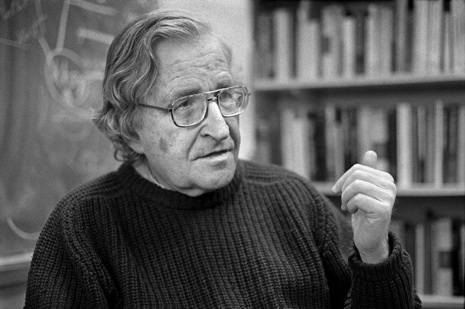
\includegraphics[width=0.4\textwidth]{images/noam-chomsky.jpg}

    {\it `But it must be recognized that the notion of ``probability of a sentence'' is an entirely useless one, under any known interpretation of this term.'}


  \end{center}
}

\pagestepalt{Could be\ldots}{
  \pause \ldots for linguistic {\it theory}.\pause 
  \begin{itemize}
  \item Humans are creative: what we can say is not directly connected
    to what we've heard in the past.\pause
  \item How we connect previous knowledge to language
    production/comprehension is still an open question.\pause
  \item But for the time being, we can ``cheat''.\pause
  \end{itemize}
  Which brings us to the topic of \alert{smoothing}.
}


\pagestepalt{So what is smoothing?}{
  Consider frequencies in language as a histogram.
  \begin{center}
    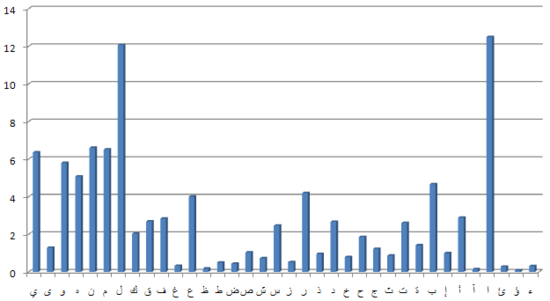
\includegraphics[width=0.7\textwidth]{images/histo.png}
  \end{center}
}

\pagestepalt{Counts that are zero make things ``bumpy''.}{
  \begin{center}
    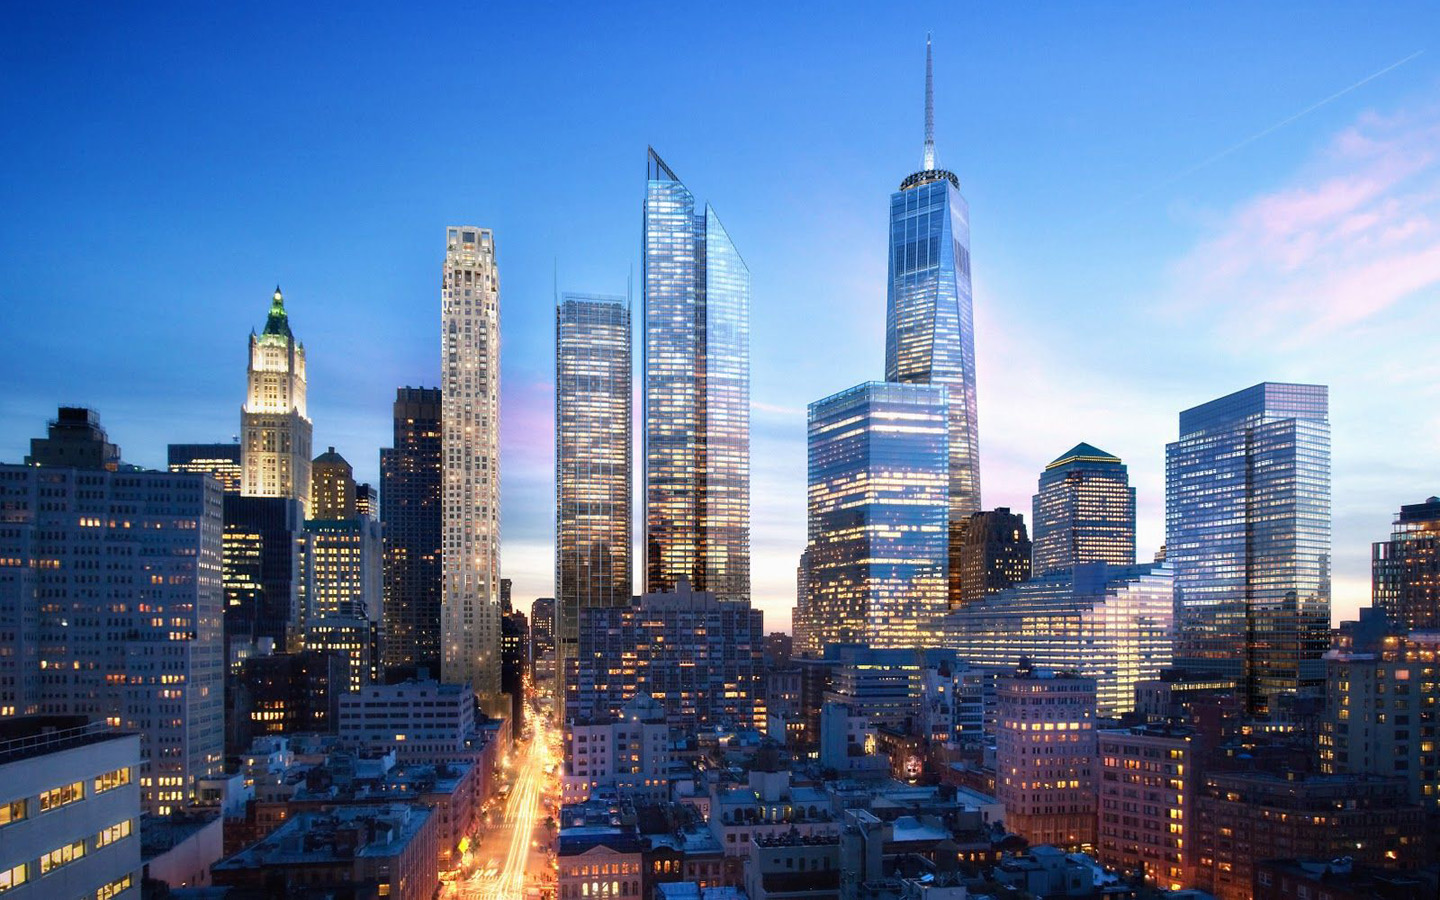
\includegraphics[width=0.6\textwidth]{images/cityskyline.jpg}
  \end{center}
  \ldots and it's just hard to do probability on bumpy distributions (as we've seen).
}

\pagestepalt{So what we want is to ``smooth'' the distribution.}{
  \begin{center}
    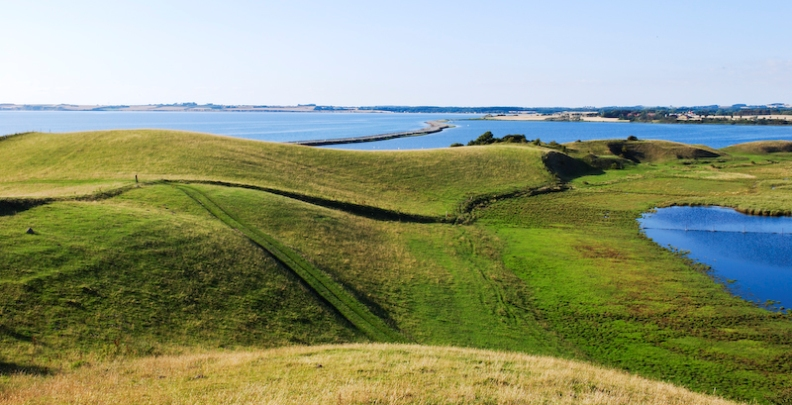
\includegraphics[width=0.8\textwidth]{images/hills.jpg}
  \end{center}
}

\pagestep{Which gives me an opportunity to talk about the sun.}{images/sunalso.jpg}

\pagestepalt{What does the sun have to do with anything?}{
  \pause It has a lot!\pause 
  \begin{center}
    \textbf{What is the chance of it not rising tomorrow?}
  \end{center}\pause
  \begin{itemize}
  \item It's always risen before.\pause
  \item But the chance of it not rising is not zero!
    \begin{itemize}
    \item ``Hard'' science fiction space disasters -- can happen!\pause
    \end{itemize}
  \item \textbf{Laplace:} how to reason about this?  Fudge the count
    of the never-seen eventuality.
  \end{itemize}
}

\pagestepalt{And hence, \alert{Laplace/add-one smoothing}.}{
  That's it.  Just add some constant.  A simple smoothing.\pause\\
  So can we solve our little sparsity problem?

  \begin{tabular}{c|cccccccc}
    word & As & much & wood & as & a & woodchuck & could & chuck\\
    \hline
    $p(w_2|w_1)$ &\alert{0}&\alert{undef}&\alert{1} & \alert{0} & \alert{undef} & \alert{1.0} & \alert{0} & 0.5 \\
  \end{tabular}  \\\pause

  \vspace{0.1cm}
  Sure we can!
  \begin{block}{Laplace smoothing}
    $p'(w_2|w_1) = \frac{count(w_1 w_2) + d}{count(w_1) + dV}$
  \end{block}
  Often we pick $d=1$, which is why it's ``add-one''.
}

\pagestepalt{Let's just add some bigram counts.}{
  We'll pick a constant of 1 and add the bigrams we need. Everything
  else gets incremented by 1.
  \vspace{-0.75cm}
  \begin{columns}[T]
      \begin{column}{0.5\textwidth}
        \begin{center}
          \small
          \begin{tabular}{c|c}
            bigram & count \\
            \hline
            (start) how & \alert{2} \\
            how much & \alert{2} \\
            much wood & \alert{2} \\
            wood could & \alert{2} \\
            could a & \alert{2} \\
            a woodchuck & \alert{3} \\
            woodchuck chuck & \alert{2} \\
          \end{tabular}
        \end{center}
      \end{column}
      \begin{column}{0.5\textwidth}
        \begin{center}
          \small
          \begin{tabular}{c|c}
            bigram & count \\
            \hline
            chuck if & \alert{2}\\
            if a & \alert{2} \\
            could chuck & \alert{2} \\
            chuck wood & \alert{2} \\
            wood ? & \alert{2} \\
            \alert{(start) as} & 1\\
            \alert{as much} & 1 \\
            \alert{woodchuck could} & 1 \\
            \alert{would as} & 1 \\
            \alert{as a} & 1 \\
          \end{tabular}
        \end{center}
      \end{column}
  \end{columns} 

  \vspace{0.1cm}
  And $V = 17$, so we can calculate our denominator.
}

\pagestepalt{We can calculate our smoothed probabilities.}{
  \begin{tabular}{c|cccccccc}
    word & As & much & wood & as & a & woodchuck & could & chuck\\
    \hline
    $p(w_2|w_1)$ &\alert{0}&\alert{undef}&\alert{1} & \alert{0} & \alert{undef} & \alert{1.0} & \alert{0} & 0.5\\
    \alert{$p'(w_2|w_1)$} & \alert{0.06} \\
  \end{tabular}  \\

  \vspace{0.1cm}
  Calculate ``(start) as'': 
  \\$p'($as$|$(start)$) =$ count'(``start as'') / (count(``start'') + 17)\\
  \\= 1/(1+17) = 0.06
  (Must use original count of start.)\\
  %\textcolor{blue}{[student exercise to compute remaining values]}
}


\pagestepalt{So now we have a sequence of bigram probabilities.}{
  \begin{tabular}{c|cccccccc}
    word & As & much & wood & as & a & woodchuck & could & chuck\\
    \hline
    \alert{$p'(w_2|w_1)$} & \alert{0.06} & \alert{0.06} & \alert{0.11} & \alert{0.05} & \alert{0.06} & \alert{0.17} & \alert{0.06} & \alert{0.11}\\
  \end{tabular}  \\

  We can now compute the probability of the sentence!\pause \\
  (Which is
  1.33e-9, a lot lower than just multiplying the nonzero unigrams,
  which was 3.76e-05.)  
}



%\placard{\textcolor{blue}{[live demo with NLTK]}}

\pagestepalt{So we've succeeded in making zero nonzero!}{
  There are still some issues for you to think about: \pause
  \begin{itemize}
  \item Is there a reason to believe that add-one smoothing is fair? 
    \begin{itemize}
    \item We did this independently of the likelihood of individual words.
%    \item In later lectures, we'll talk about Good-Turing estimation,
%      Kneser-Ney, and so on.
    \end{itemize}
  \item  Add-one smoothing is not typically used.\pause
    \begin{itemize}
    \item It's very aggressive! It ``steals'' too much probability mass from 
      things we've actually seen.\pause
    \item Not all {\it hapax legomena} are equally likely.\pause
  \end{itemize}
  \item \textbf{Are there better ways to do it?}
  \end{itemize}
}


\begin{frame}{Discounting: an interlude}
  \begin{center}
    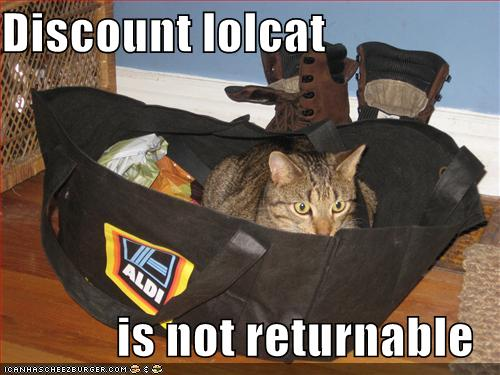
\includegraphics[scale=0.2]{images/discount.jpg}
  \end{center}
  
  Before we move on\ldots there's another way to look at add-one: 
  in terms of a \textbf{discount}.
  \begin{block}{Add-one discount formula}
    \[d_c = \frac{c^*}{c}\]
  \end{block}
  This tells us how much we ``stole'' from a word with original count $c$
  in order to give to the unseen forms.
\end{frame}

\begin{frame}{Good-Turing discounting}
  In add-one smoothing:\pause
  \begin{itemize}
  \item We pretend we've seen unknown n-grams \textbf{once}. \pause
  \item We don't take into account what effect it will have on the 
    other n-grams.\pause
  \item We compensate for it in a VERY crude manner.\pause
  \end{itemize}
  We can do better: 
  \begin{itemize}
  \item We can START by estimating how likely it is we're going to see
    something new.
  \end{itemize}
\end{frame}


\begin{frame}{Good-Turing discounting}
  \begin{block}{Insight}
    The number of things we've never seen can be estimated from the
    number of things we've seen only once.
  \end{block} \pause
  But THEN, that means that we have to steal probability from everyone
  else.  \pause
  \begin{itemize}
  \item How to do that fairly?\pause
  \item We need to reestimate the probability of \textbf{everything} 
    by the same principle.  
  \end{itemize}
\end{frame}

\begin{frame}{Good-Turing discounting}
  Key concept: \textbf{frequency of frequency}.
  \begin{itemize}
  \item $N_c$ --- how often n-grams of frequency $c$ appear in the corpus.
  \end{itemize}\pause

  \begin{block}

    \[N_c = \sum_{x:\mathrm{count}(x)=c} 1\]
  \end{block}\pause

  Then we can compute revised counts for everything.
  \begin{block}

    \[c^* = (c+1)\frac{N_{c+1}}{N_c}\]
  \end{block}
\end{frame}


\begin{frame}{Good-Turing discounting}
  So how do we get the probability of missing items?\pause
  \begin{block}

    \[P^*_{GT}(\mathrm{count}(w) = 0) = \frac{N_1}{N}\]
  \end{block}
  Where $N$ is the total number of tokens.\\
  (I'll leave proof as an exercise for the reader.)
\end{frame}


\begin{frame}{Issues with Good-Turing}
  Some things to note:
  \begin{itemize}
  \item Assumes that the distribution of each bigram is binomial.\pause
    \begin{itemize}
    \item If you have a vocab $V$, then the number of bigrams is $V^2$, 
      so what happens to OOV words?\pause
    \end{itemize}
  \item What happens when we don't know $N_{c+1}$? \pause
    \begin{itemize}
    \item We have to smooth out the frequency of frequency counts!
    \end{itemize}\pause
  \item We don't necessarily discount things where the count is big:
    probably reliable.\pause
    \begin{itemize}
    \item But everything must sum to 1!
    \end{itemize}
  \end{itemize}
\end{frame}

\begin{frame}
  \begin{center}
    \huge
    So far we've focused mostly on bigrams. But what about bigger ``grams''?
  \end{center}
\end{frame}

\placard{This raises an important question.}

\pagestep{Why cats smooth.}{images/622119.jpg}

\begin{frame}{Higher-order n-grams}
  What about ``why cats smooth''?\pause
  \begin{itemize}
  \item Not frequent enough to appear in Google n-grams.\pause
  \item But maybe the bigrams will help us: ``why cats'' and ``cats smooth''.
  \end{itemize}\pause
  And even if bigrams don't help us, maybe some other combination will
  get us a more realistic estimate.
\end{frame}

\begin{frame}{Interpolation}
  So what we want to find is $P(w_n|w_{n-2}w_{n-1})$ --- that's 
  the definition of the probability of a trigram.\pause
  \begin{block}{Linear interpolation}
    \[\hat{P}(w_n|w_{n-2}w_{n-1}) = \lambda_1 P(w_n|w_{n-2}w_{n-1})\]
    \[+ \lambda_2 P(w_n|w_{n-1}) + \lambda_3 P(w_n)\]
  \end{block}\pause
  Then we just need to learn the $\lambda$ weights (by EM or 
  any other linear regression trick).\\\pause
  We can also make the weights context-dependent by making them relative
  to bigrams.
\end{frame}

\begin{frame}{Backoff}
  An even better way: \textbf{Backoff}
  \\ For example, Katz (haha!) backoff.
  \begin{block}{}   
    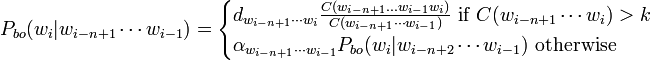
\includegraphics[width=\textwidth]{images/katzP.png}
  \end{block}
  \begin{block}{}
    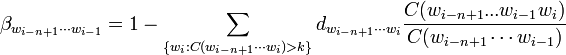
\includegraphics[width=\textwidth]{images/katzB.png}
  \end{block}
  \begin{block}{} 
    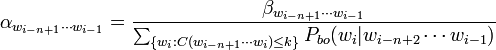
\includegraphics[width=\textwidth]{images/katzA.png}
  \end{block}
\end{frame}

\begin{frame}{Katz backoff}
  \ldots but that's kind of ugly-looking. What it's really saying is that:\pause
  \begin{itemize}
    \item Use the discounted weight if the count of the n-gram in question 
      is acceptably large.\pause
    \item If not, use the n-minus-1-gram's count, adjusted by a 
      special $\alpha$ factor that adjusts the count to include 
      the mass you lost by excluding one word.\pause
    \item You calculate THAT using all the n-minus-1-grams that
      involve the word you dropped.
  \end{itemize}
\end{frame}

\pagestepalt{So just a couple of final thoughts.}{
  \begin{itemize}
  \item Is there a better way to estimate n-gram probabilities in the first place?\pause 
  \item Are n-grams and smoothing a good model of sentences? Where are they 
    deficient?
  \end{itemize}
}




\pagestepalt{The End.}{
  \begin{center}
    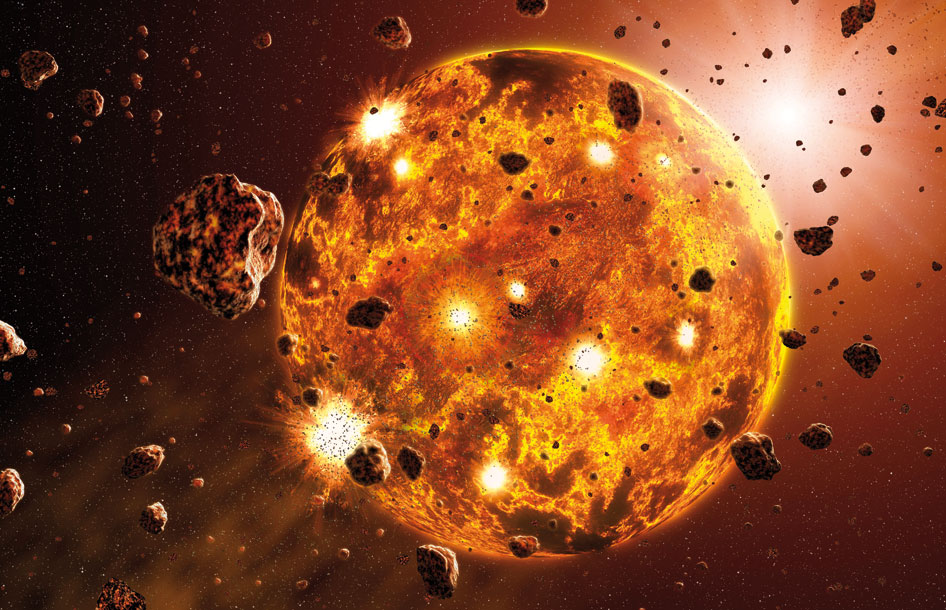
\includegraphics[width=0.8\textwidth]{images/formation.jpg}
  \end{center}
}

\end{document}
